\documentclass[12pt]{article}
\newcommand{\ts}{\textsuperscript}

\usepackage[margin=1in]{geometry}
\usepackage{caption}
\usepackage{cite}
\usepackage{subcaption,graphicx}
\usepackage{lineno, blindtext}
\usepackage{float}
\usepackage{color}
\usepackage{graphicx}
\usepackage[hidelinks]{hyperref}
\usepackage{enumitem}
\usepackage{multicol}
\usepackage{fancyhdr}
\usepackage{times}
\usepackage{mathtools}
\usepackage{pdfpages}
\setlength{\parindent}{0pt}
\newcommand{\forceindent}{\leavevmode{\parindent=1em\indent}}
%\usepackage{siunitx}
\usepackage{chronology}

\title{\textbf{MSE 450\\Project Proposal\\Real-Time Embedded Control System\\ for an Inverted Pendulum}}
\author{\\ \\ \\Self Proposed Project Group 1\\ Rachel George -  301288581 \\ Ryan Fielding - 301284210}
\date{March $9^{th}$, 2020}

\begin{document}

\maketitle
\newpage

{\Large \textbf{Abstract\\\\}}
This report outlines the project proposal for the MSE 450 (Real-time and Embedded Control Systems) course project, which will be developed in conjunction with the MSE 483 (Modern Control Systems) course project. In short, the system will implement a state space model feedback control system via the course Tiva C TM4C123GH6PM microcontroller, with the goal of stabilizing an inverted pendulum across various small impulses. This inverted pendulum system will be built from the parts of a broken Canon printer donated by a past high school teacher. The main components taken from this printer include the printer cartridge track (for the cart), a DC motor, linear optical encoder. The pendulum will be mounted to a potentiometer to measure the angle of the pendulum, which will be mounted to the cart, whose position will be measured (inc/decremented) by the optical encoder. To effectively implement this system, the Tiva C microcontroller initialization must be completed early on, in order to allow for state model controller testing and to ensure a stabilized pendulum by the project deadline. The initialization will consist of:
\begin{itemize}
\item 2 digital inputs for the optical quadrature encoder outputs, A and B, which will increment and decrement the cart position via interrupts.
\item 1 analog input for the angle of the pendulum via a 10k$\Omega$ potentiometer.
\item 2 PWM outputs for the actuation and control of the 12V, 1A DC motor through an H-bridge (TA7267BP) interface board, connected to the cart via a belt drive.
\end{itemize}
Initialization of the microcontroller and all working components will be completed by March $15^{th}$, 2020, to allow enough time for state model development and testing. This includes but is not limited to, measurement of $\theta \textrm{ and } x$, ensuring that the position increments properly at high speeds, and adequate position control of the DC motor powered cart. At this point, the observer based state feedback controller can be implemented. The final control system will be complete and tested by March $30^{th}$, 2020.

\newpage
\tableofcontents
\listoffigures
\newpage

\section{Introduction}
\subsection{Overview}
The system discussed from a controls perspective, involves the concept of an inverted pendulum; an unstable system which if otherwise not intervened with by engineered calculated actuation, will become unbalanced due to gravity and the displacement of the pendulum's centre of gravity from a set point. This experiment encapsulates a true real-time system which integrates an embedded computer system to react within stringent response-time constraints. 
\\\\
Physically the system will be built of reused spare parts from a broken Canon printer, donated from one of the team member's previous high school teachers. Parts salvaged include a linear guide rail, a 12V, 1A DC motor and a linear optical encoder. A basic potentiometer will be used to measure the angle of the pendulum. The platform chosen to control this system is the Tiva TM4C123GH6PM microcontroller. It will be integrated with an H-bridge motor interface board to drive the DC motor, and the outlined sensors. Software development will be done in Code Composer Studio written in C.
\subsection{Control System Background}
The controller's commands will be dependent on the feedback of the state system; this ultimately entails a closed loop system. As exemplified below (Figure \ref{fig:loops}), it is the difference between a closed loop system and an open loop system. Simply put, an open loop system has no indication of its perpetuated error that it may be incurring, therefore feedback loops or closed loop systems can respond accordingly to disturbances that deviate the output from the target value.
\begin{figure}[H]
    \centering
    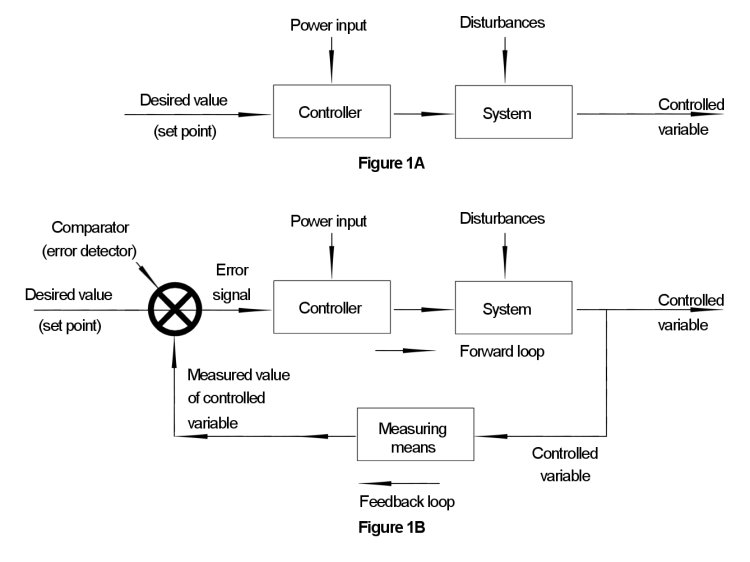
\includegraphics[width=.70\linewidth]{figures/closedopenloop.jpg}
    \caption{Open Loop System Versus a Closed Loop System \cite{OCLoop}}
    \label{fig:loops}
\end{figure}

\subsection{Problem Investigation}
The measure of a successful closed-loop system is merited by its degree to which the measured final value compares to its target value after the system responds to a disturbance. This success can be measured by multiple characteristics of the system response. One such characteristic is the maximum error, a value which corresponds to the initial overshoot of the system response \cite{OCLoop}. Another valuable criteria is the response time and the settling time of the  system; the time from which an error is detected to when a corrective action is taken, and the time taken for the controller to complete its corrective path, respectively. After the final value is obtained, the steady state error is observable - the absolute difference of the final measured value and the ideal value, see the figure below for this visual representation (Figure \ref{fig:Resp}).
\begin{figure}[H]
    \centering
    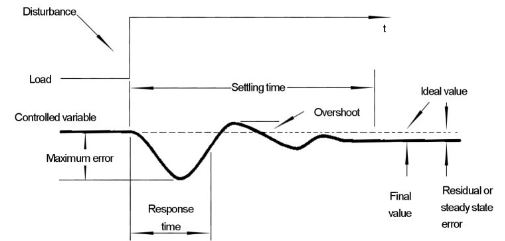
\includegraphics[width=.7\linewidth]{figures/System response.JPG}
    \caption{System Measurement - System Response to Disturbances  \cite{OCLoop}}
    \label{fig:Resp}
\end{figure}

State Space Modelling will be implemented as the chosen model, ergo using the "notations of state, inputs, outputs and dynamics to describe the behavior of a system"\cite{StateSpace}. From the perspective of an unstable system, state modelling will allow us to predict the behavior of the system. Partner this with real time feedback, and one is able to implement a state feedback controller to achieve a desired objective. In our case, stabilization of an inverted pendulum.

\subsection{Expected Outcome(s)}
We expect to obtain a system response and from observing its characteristics previously explained, we plan to manipulate the system to minimize the steady state error. This error  responds to a system gain, however it is important to balance the increase of gain to the system as it impacts the sensitivity of the response and may additionally result in the increase of the maximum error and/or settling time \cite{OCLoop}. A critically damped system with a medium gain is most desirable. This can be observed through an ideal physical system producing minimum oscillation about the set point to counteract the moment created by the movement of the pendulum's center of mass. From this experiment we also aim to form a solidified concept of embedded computer control system programming; designing and building a system, integrating hardware and software for an embedded control application.

\section{Design Goals and Objectives}
\subsection{Objectives}
The goal of this controller aims to maintain the pendulum in a state of inversion, that is, an angle of $\theta = 180^o$, constantly and for various impulse forces to the pendulum, by changing the position ($x$) of the cart. See figure \ref{fig:pend} below.
\begin{figure}[H]
    \centering
    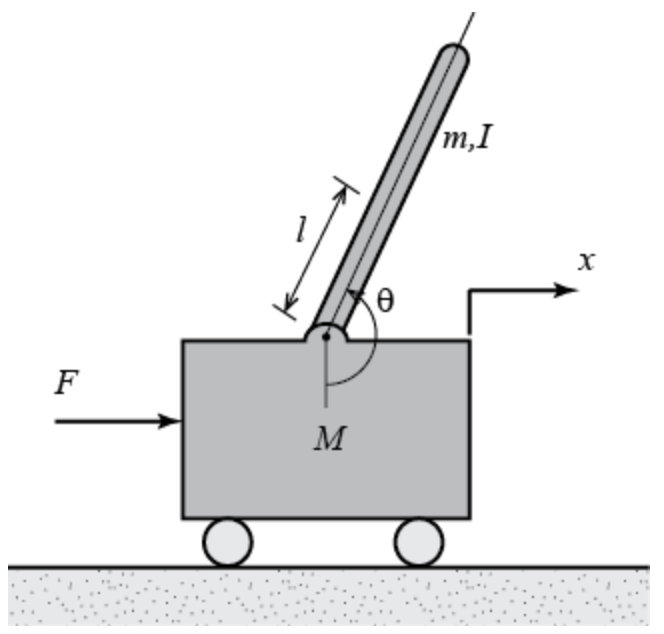
\includegraphics[width=.4\linewidth]{figures/pend.png}
    \caption{System Concept - Inverted Pendulum on a Cart \cite{inv}}
    \label{fig:pend}
\end{figure}

\textbf{Variables}
\begin{itemize}
    \item $x$ the position of the cart
    \item $\theta$ the angle of the pendulum
    \item $F$ applied forces to the cart
    \item $M, m$ masses of the cart, pendulum
    \item $l, I$ length and inertia of the pendulum
\end{itemize}
\subsection{Nice to Have's}
\label{nice}
In addition the the objectives outline in the previous section, there are many sub-features that can be developed in the software of this system that present complex control theory problems, 2 of which are outlined below.
\begin{itemize}
    \item Side-stepping of cart to a desired position ensuring constant pendulum stability.\\ \indent - For example, move cart from $x=0cm$ to $x=10cm$ with minimal overshoot, rise time, steady state error.
    \item Swing-up and swing-down commands\\ \indent - Enables the system to move the cart from one state of stability to another, ie. from $\theta =0^o$ to $\theta =180^o$ and stabilize, or vice versa with minimum oscillation.
\end{itemize}
\section{Requirements and Methods}
\subsection{Control Model}
MSE 483 - Modern Control Systems / Intro to State Space Control Systems - effectively outlines the process of implementing a state space model based control system. Physical systems possess many non-linearities and thus more practical models and tuning will need to be implemented. Such as the problem of the nonlinear control of an inverted pendulum, which sees to balance the pendulum from an unstable equilibrium position. Such controls methods include Linear Quadratic Regulation (LQR), observer based state feedback control and more. The following flowchart displays the proposed observer based state feedback control model, implementing an observer due to the fact that the system does not provide full state feedback, which would require the purchase of 2 tachometers to measure the rate of change of $\theta, x$, that is, $\dot{\theta}, \dot{x}$. However, we will be implementing a state estimator to estimate the values of these states instead.
\begin{figure}[H]
    \centering
    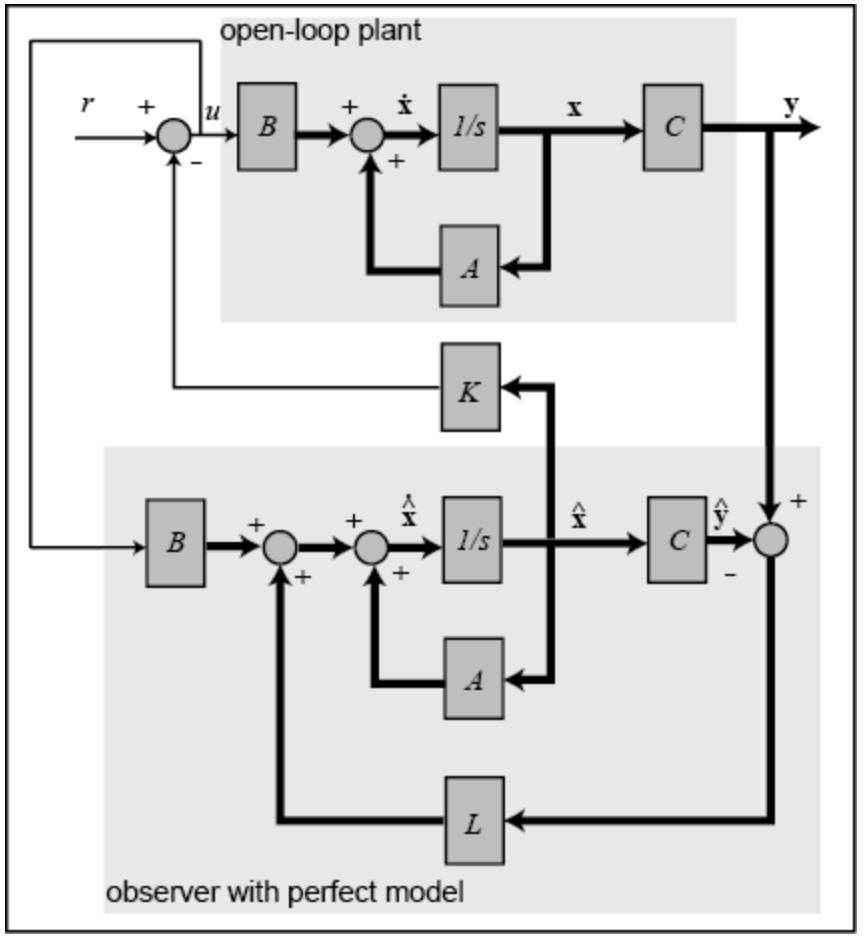
\includegraphics[width=.5\linewidth]{figures/flow.png}
    \caption{Flow Chart - Predicted State Feedback Model to be Implemented \cite{inv2}}
    \label{fig:fc}
\end{figure}
The above control system will not be elaborated too in depth as it is out of the scope of this report, however it presents the overall concept. The most important variables and what they represent are discussed in the following:
\begin{itemize}
    \item $x$ the states of the system - $x, \dot{x}, \theta, \dot{\theta}$, measured and estimated through observer based state feedback.
    \item $y$ the demanded outputs of the controller, $x, \theta$
    \item $u$ the inputs to the system, which would be the force to the cart, $F$.
    \item All other matrices, $A, B, C, D$ and so forth, represent the complete state model for the linearized system, full form shown below:
\end{itemize}
\begin{equation}
    \dot{x} = Ax + Bu \textrm{ and }
    y = Cx + Du
\end{equation}
And for the state estimator:
\begin{equation}
    \dot{\hat{x}} = A\hat{x} + Bu + L(y-\hat{y}) \textrm{ and }
    \dot{e} = \dot{x} - \dot{\hat{x}} = ... \implies \dot{e} = (A - LC)e
\end{equation}

\subsection{Experimentation}
To evaluate the proposed control models, experimentation will roughly proceed as follows:
\begin{enumerate}
    \item Power on the microcontroller with latest code developments.
    \item Normalize the cart position and pendulum angle (move cart to center of guide rail, hold pendulum vertically).
    \item Release the pendulum and evaluate controller effectiveness / stability.
    \item Introduce minor disturbances to the pendulum and the cart, evaluate system response.
\end{enumerate}
    
\subsection{Requirements}
The requirements for this problem are short and sweet - to balance the pendulum vertically as opposed to letting it fall over due to gravity. To elaborate on these requirements, we can set the following parameters:
\begin{itemize}
    \item $\Delta \theta < 1^o$ for small impulses to the pendulum or cart.
    \item Settling time of $< 4$ seconds.
    \item Cart position must be settled consistently at a constant location, ie. $x=0cm$.
\end{itemize}
Further requirements may be set for the Nice to Have's outlined in section \ref{nice}, depending on the project's completion schedule. Assuming all prior requirements are complete, we will investigate said problems and construct design requirements. 
\section{Platform and Tools}
\subsection{Hardware}
The Tiva TM4C123GH6PM microcontroller from Texas Instruments will be used as the real-time embedded controller. Code Composer Studio 9.3.0 for Mac OS X will be used to program and debug the board.\\ \par
As for the hardware of the inverted pendulum system, the re-purposed Canon printer can be seen throughout the following figures.

\begin{figure}[H]
\centering
\begin{subfigure}{.5\textwidth}
  \centering
  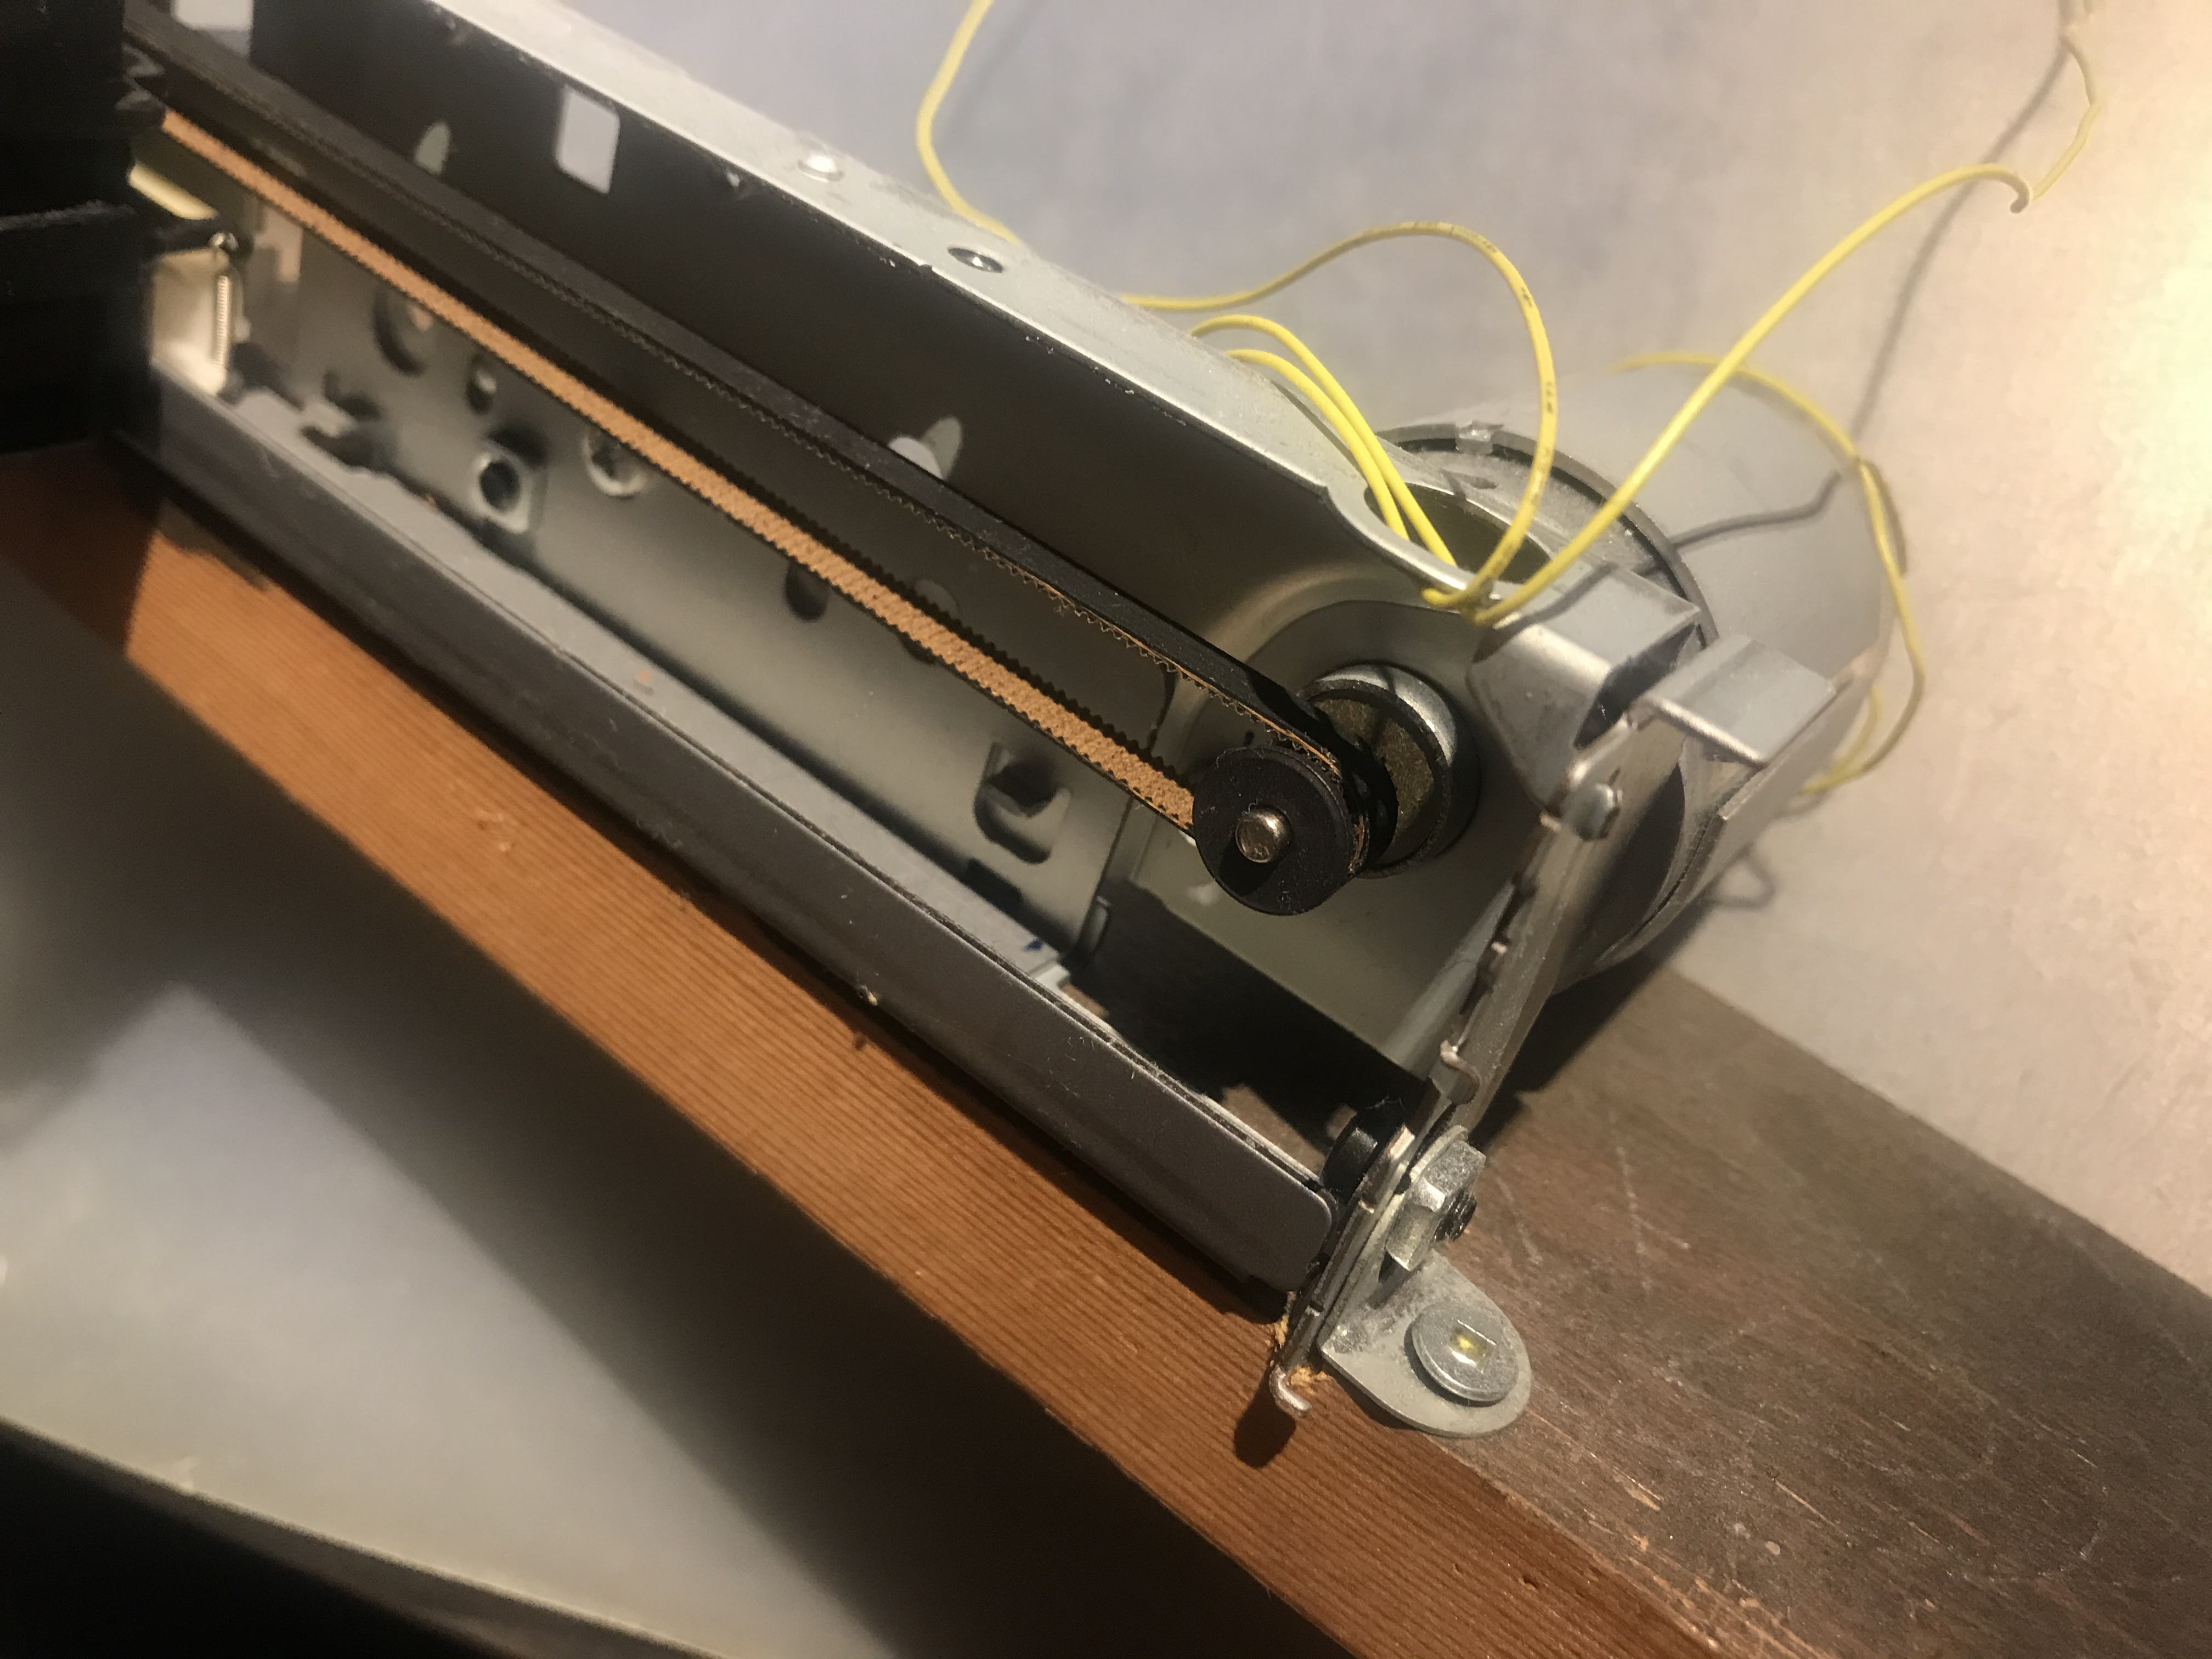
\includegraphics[width=1\linewidth]{figures/IMG_5674.jpg}
  \caption{DC Motor Belt Drive}
  \label{fig:dc}
\end{subfigure}%
\begin{subfigure}{.5\textwidth}
  \centering
  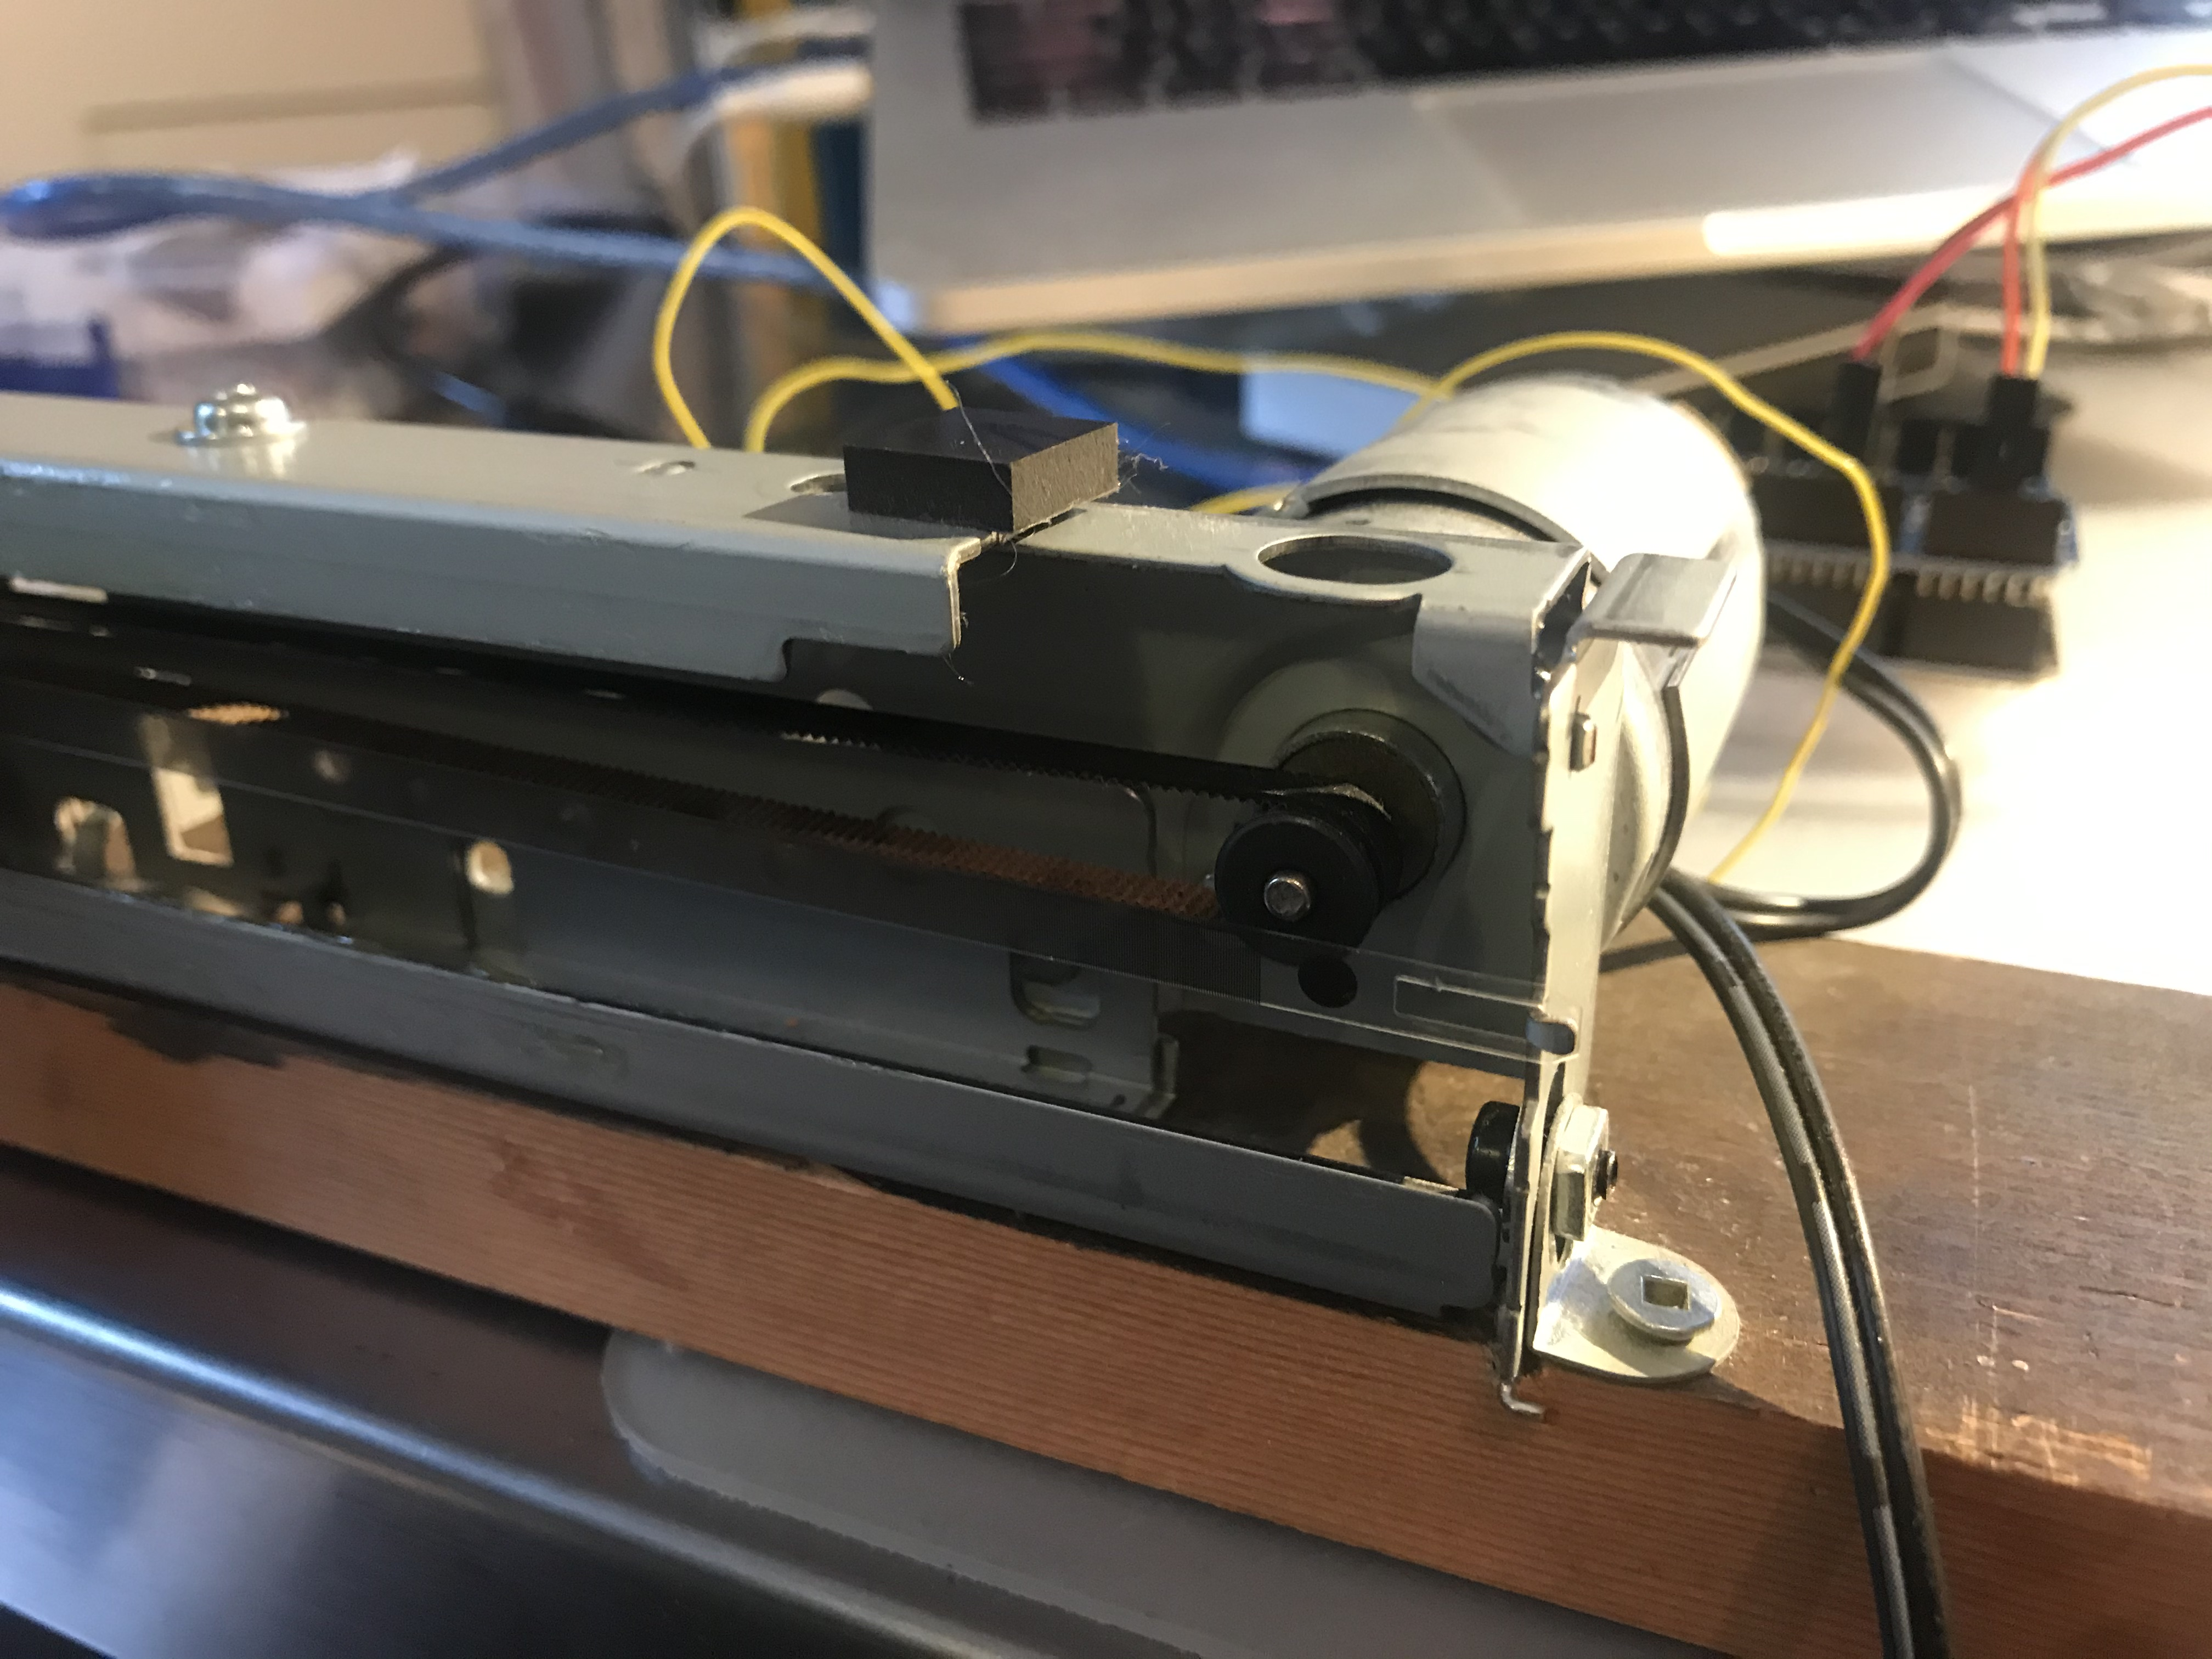
\includegraphics[width=1\linewidth]{figures/IMG_5807.jpg}
  \caption{Optical Encoder Linear Strip}
  \label{fig:opt}
\end{subfigure}
\caption{DC Motor Belt and Feedback}
\end{figure}

\begin{figure}[H]
\centering
\begin{subfigure}{.5\textwidth}
  \centering
  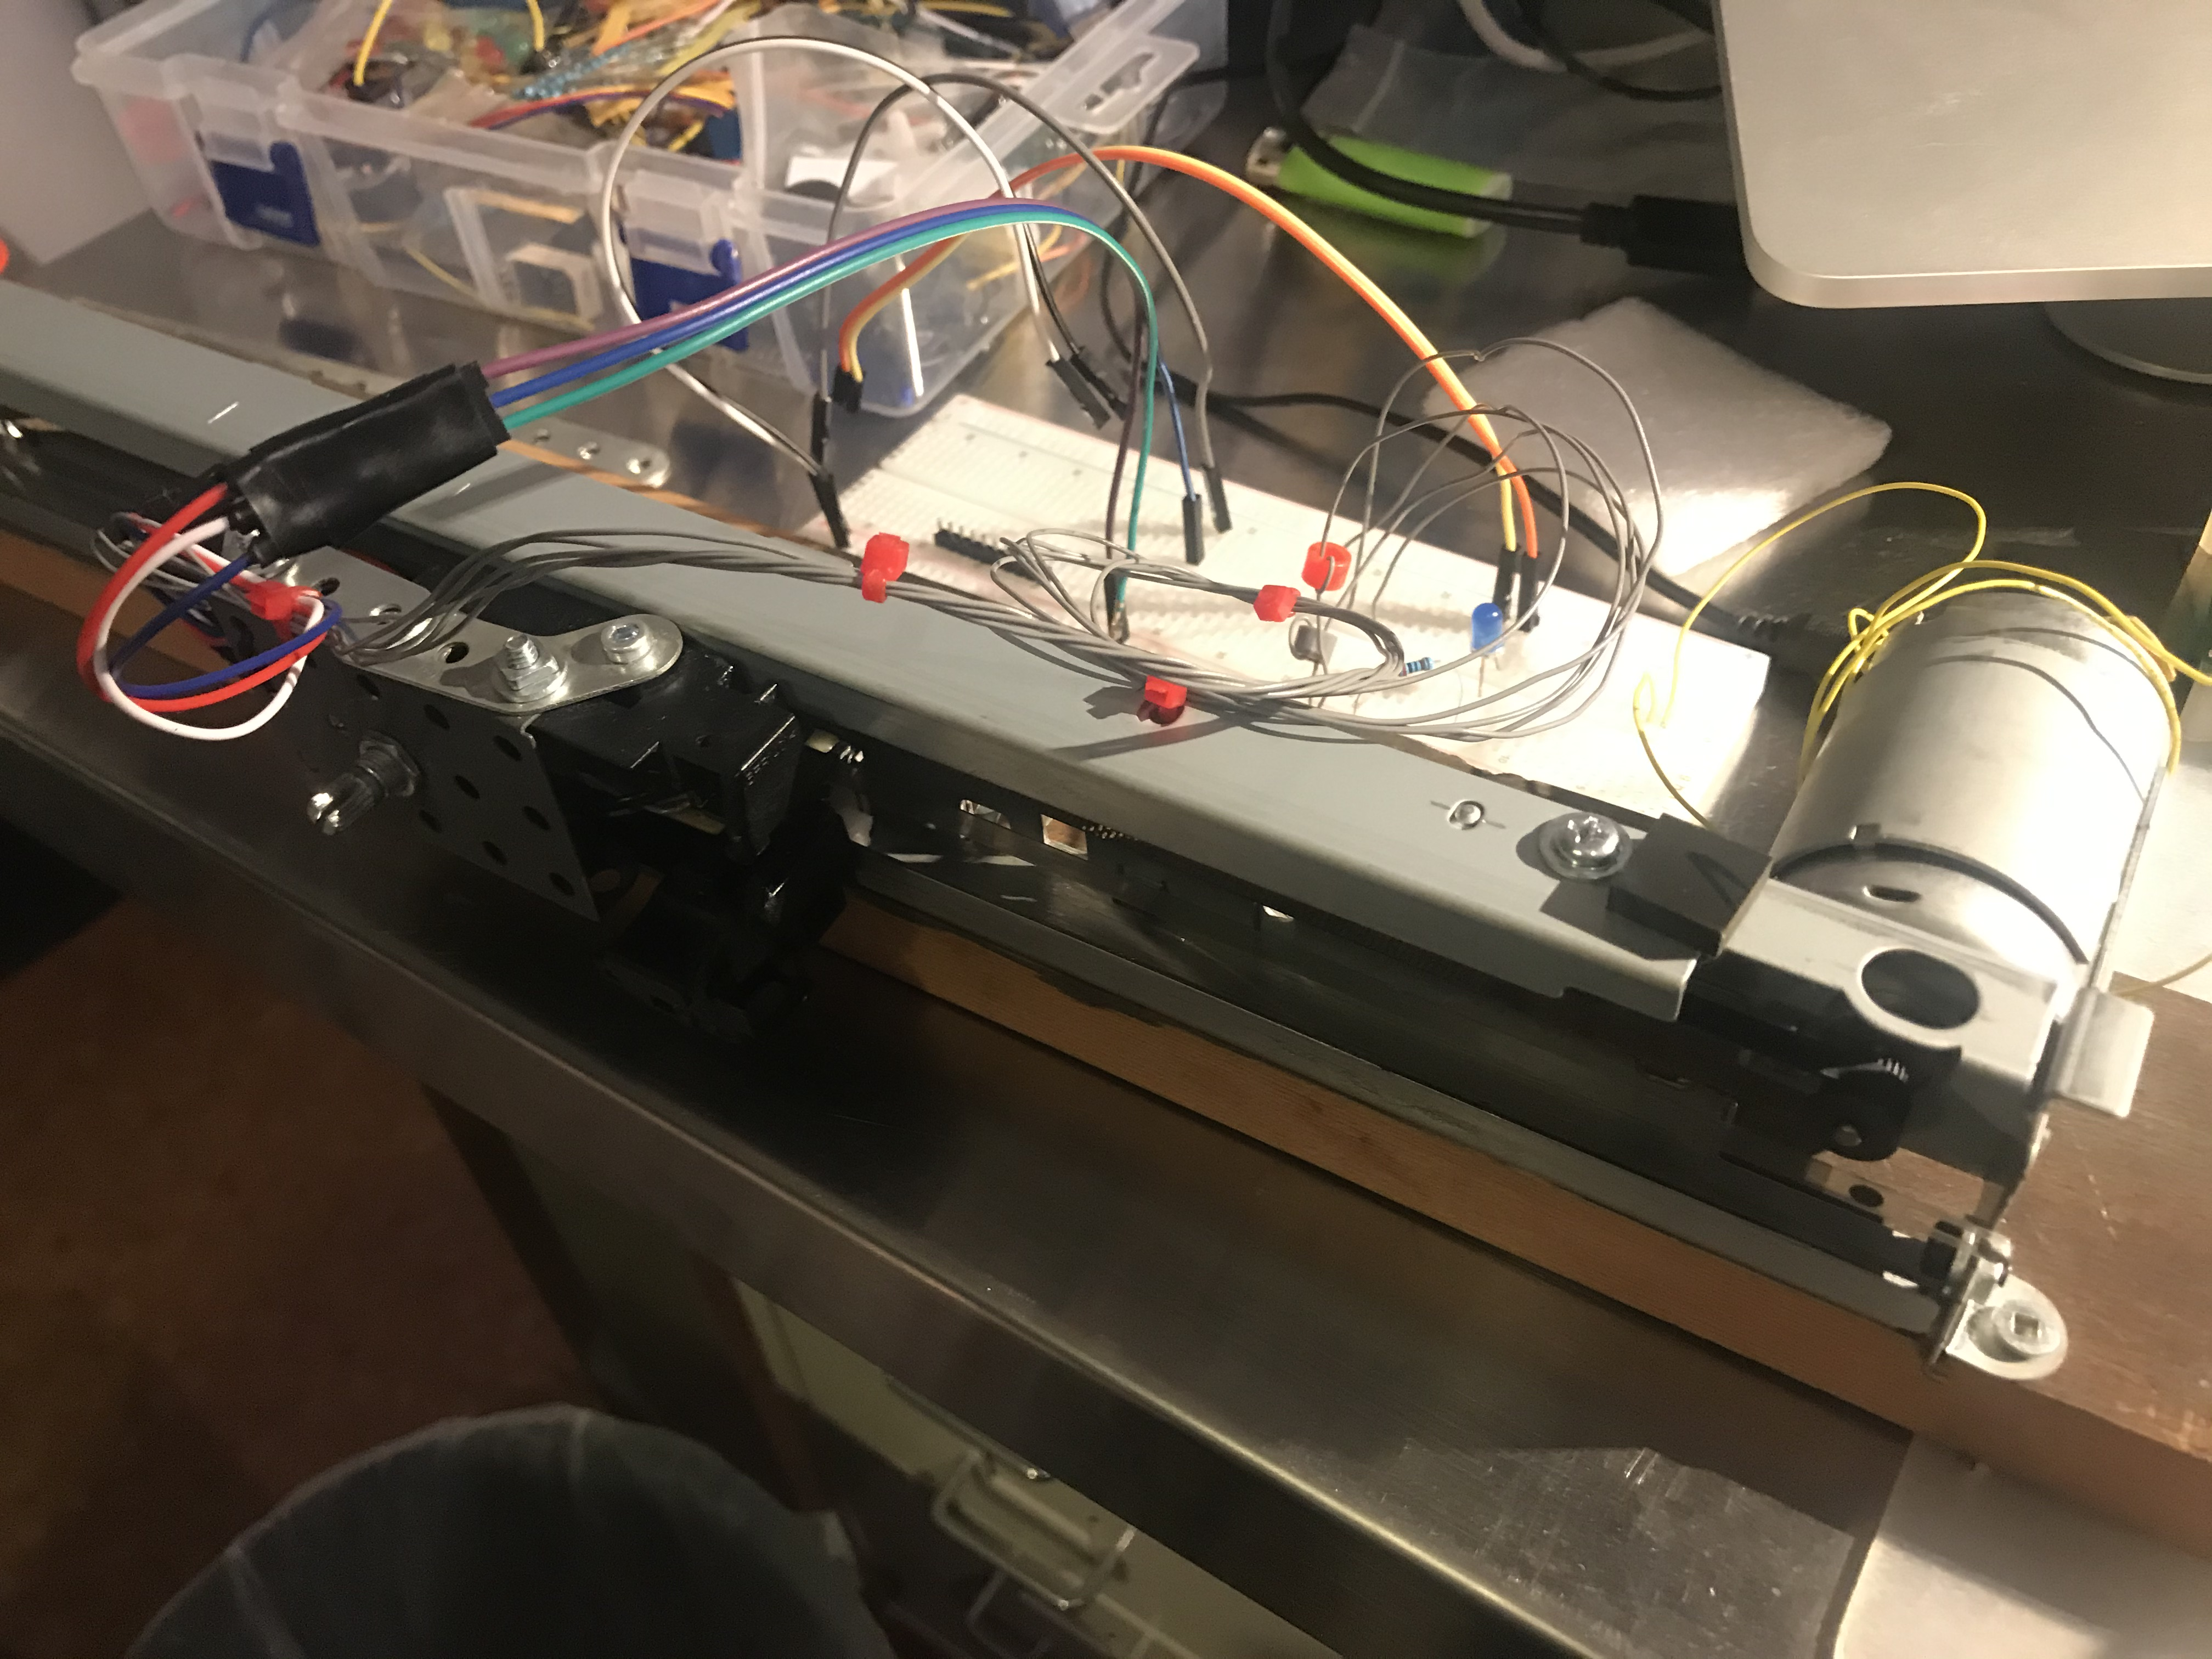
\includegraphics[width=1\linewidth]{figures/IMG_5831.jpg}
    \caption{System Setup with Wiring}
    \label{fig:wire}
\end{subfigure}%
\begin{subfigure}{.5\textwidth}
  \centering
  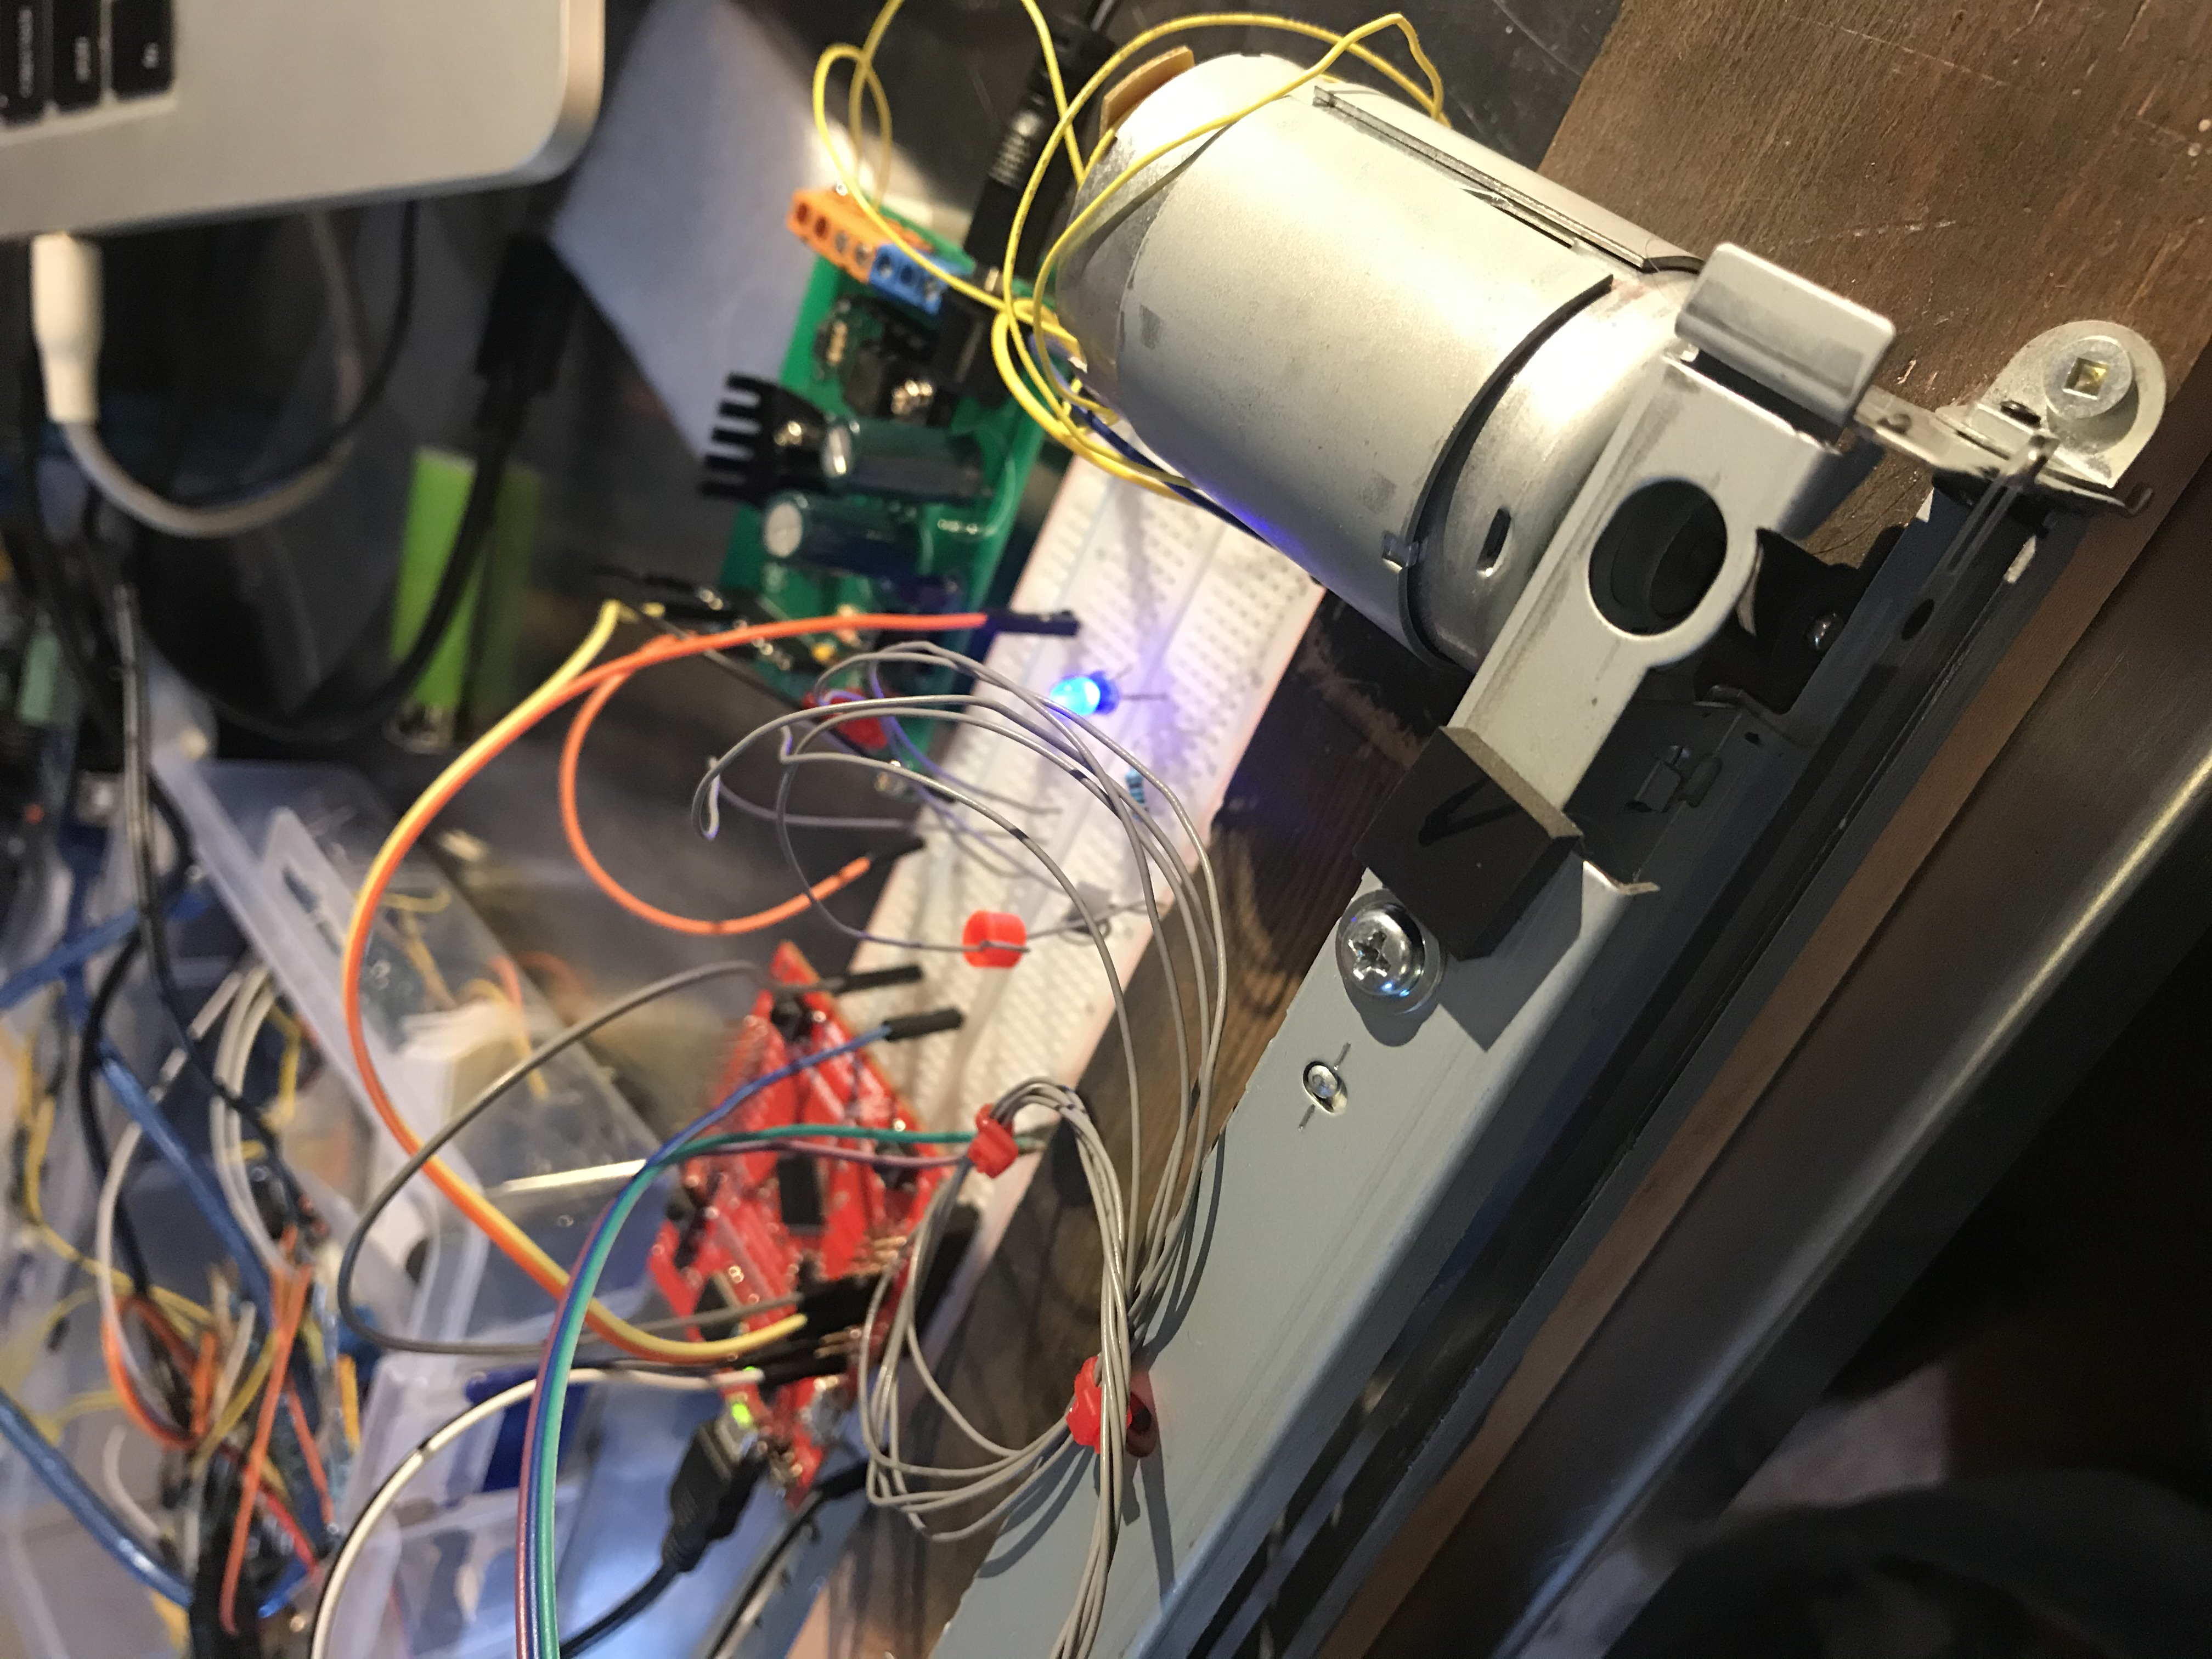
\includegraphics[width=1\linewidth]{figures/IMG_5848.jpg}
    \caption{System Electronics}
    \label{fig:elec}
\end{subfigure}
\caption{System Setup}
\end{figure}

\begin{figure}[H]
\centering
\begin{subfigure}{.5\textwidth}
  \centering
  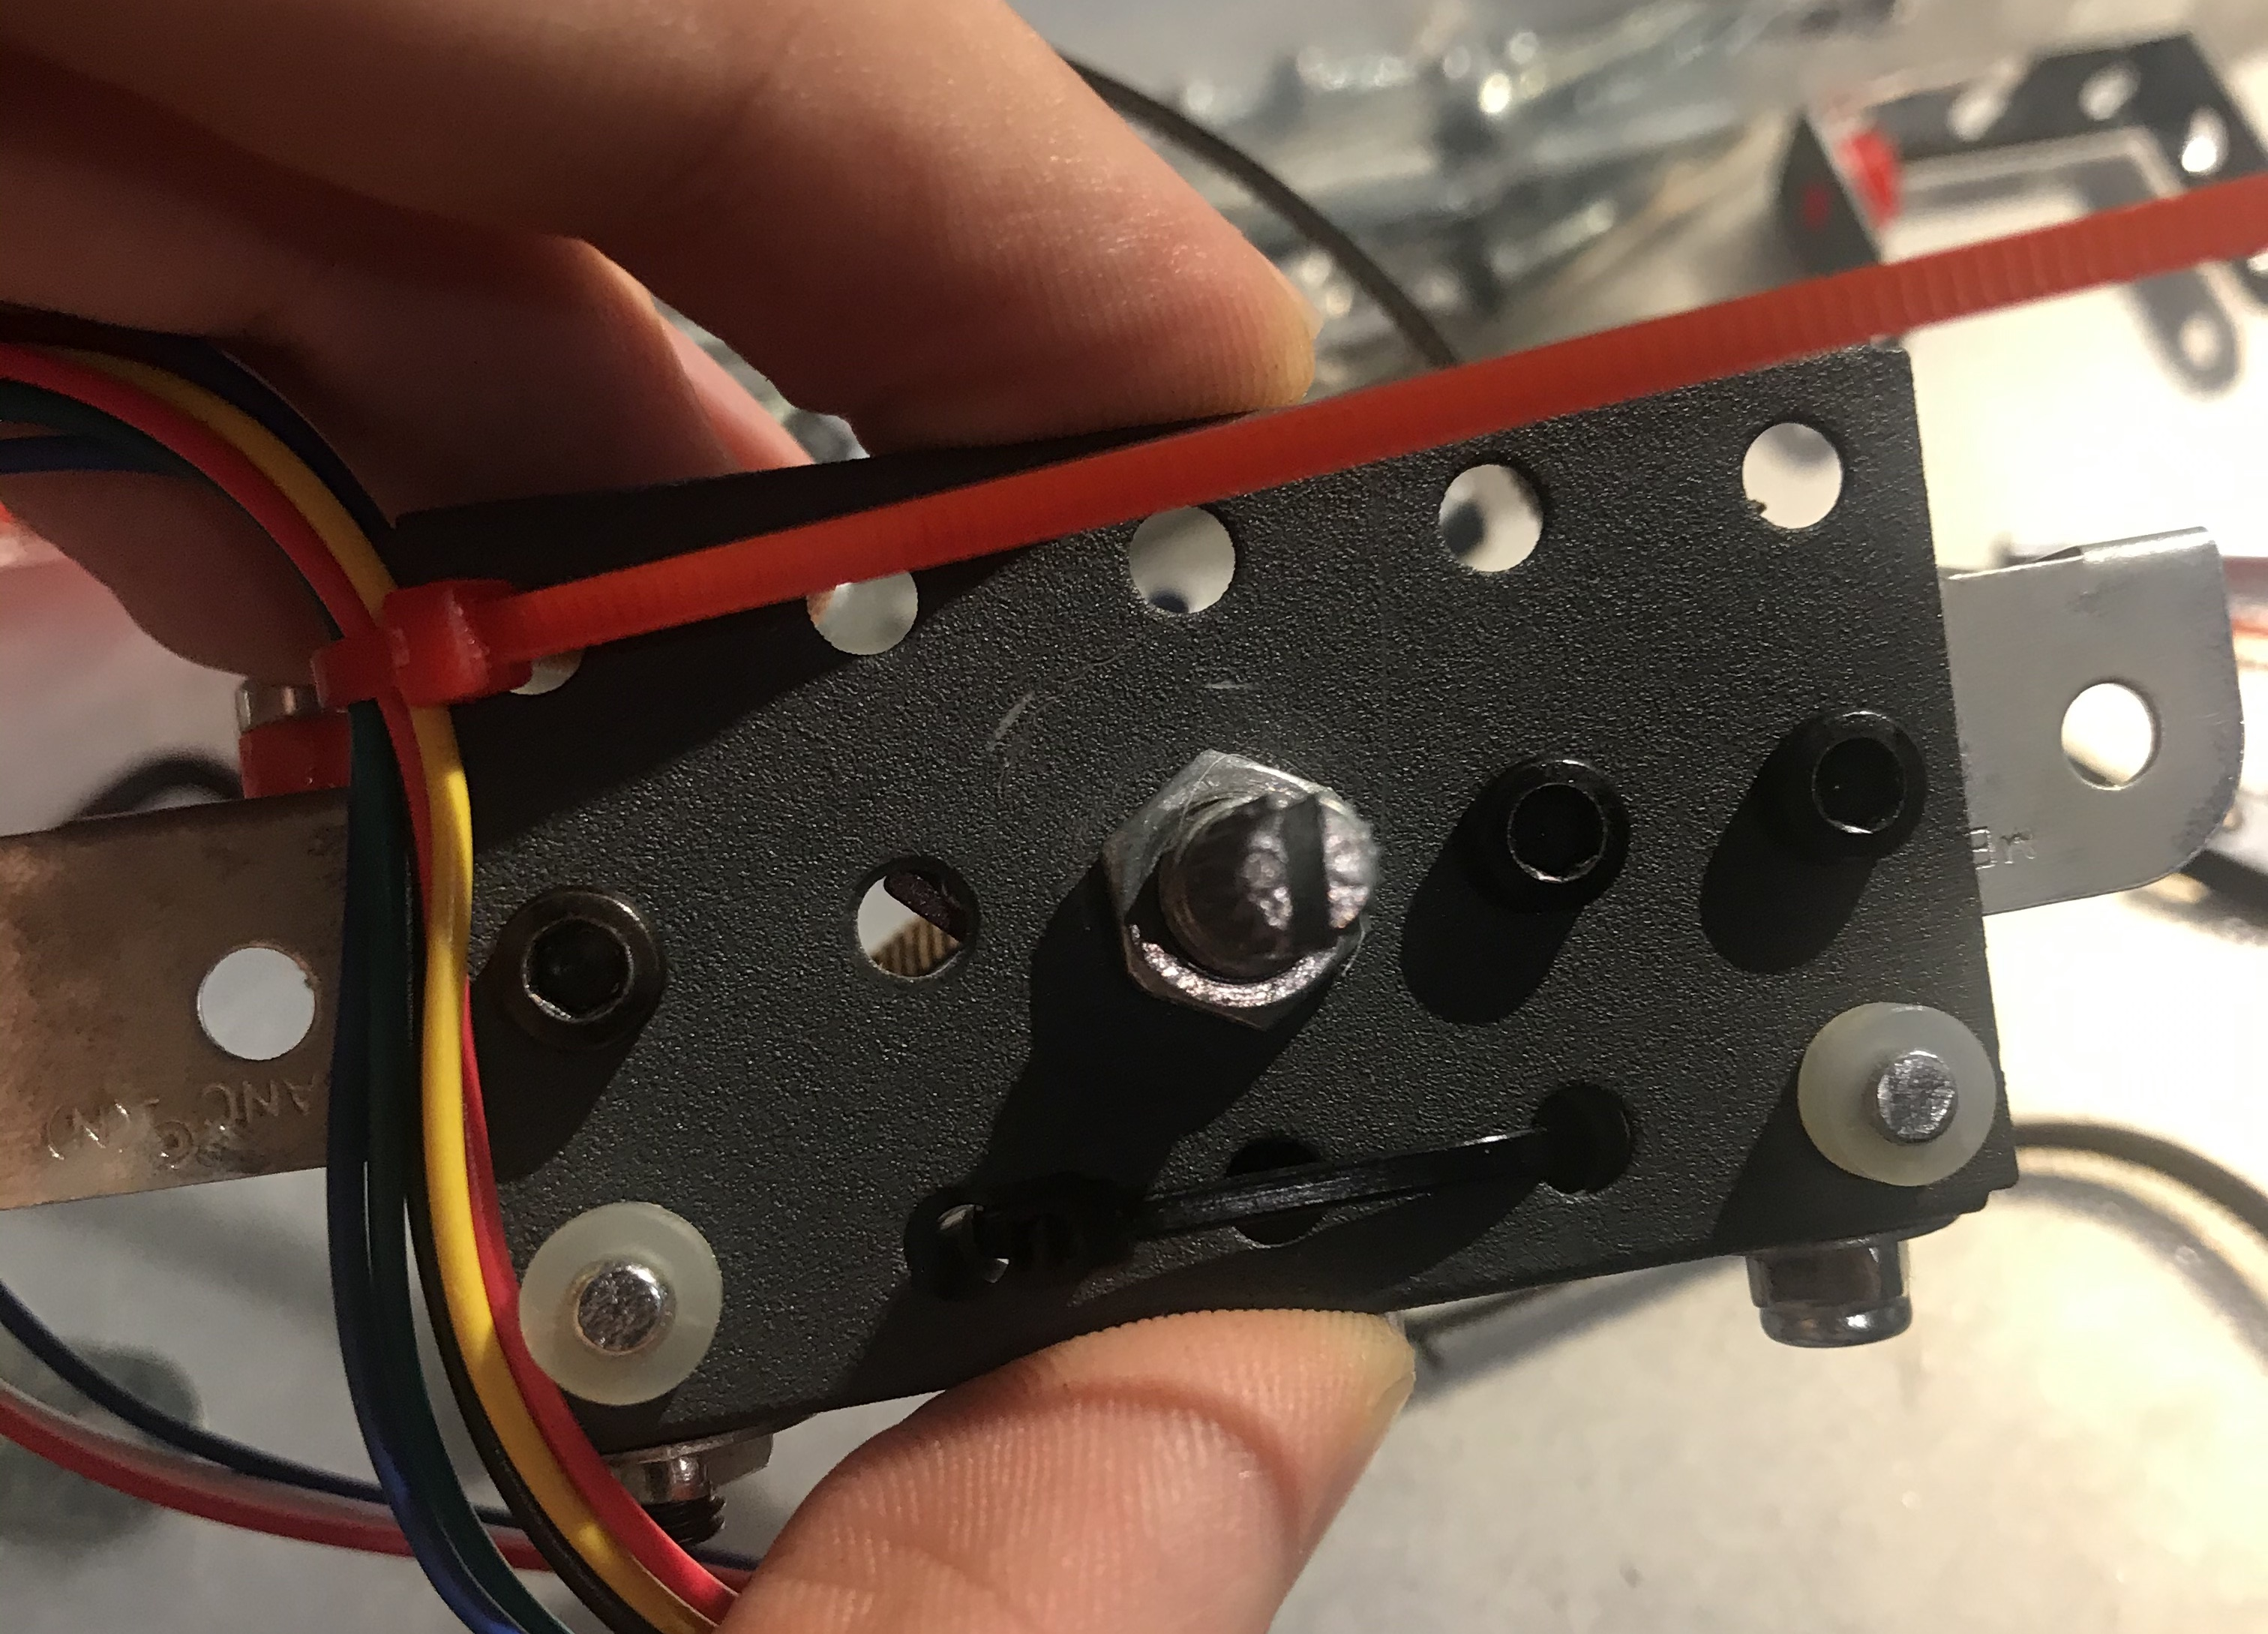
\includegraphics[width=1\linewidth]{figures/IMG_5874.jpg}
  \caption{Potentiometer on Cart}
  \label{fig:cart}
\end{subfigure}%
\begin{subfigure}{.36\textwidth}
  \centering
  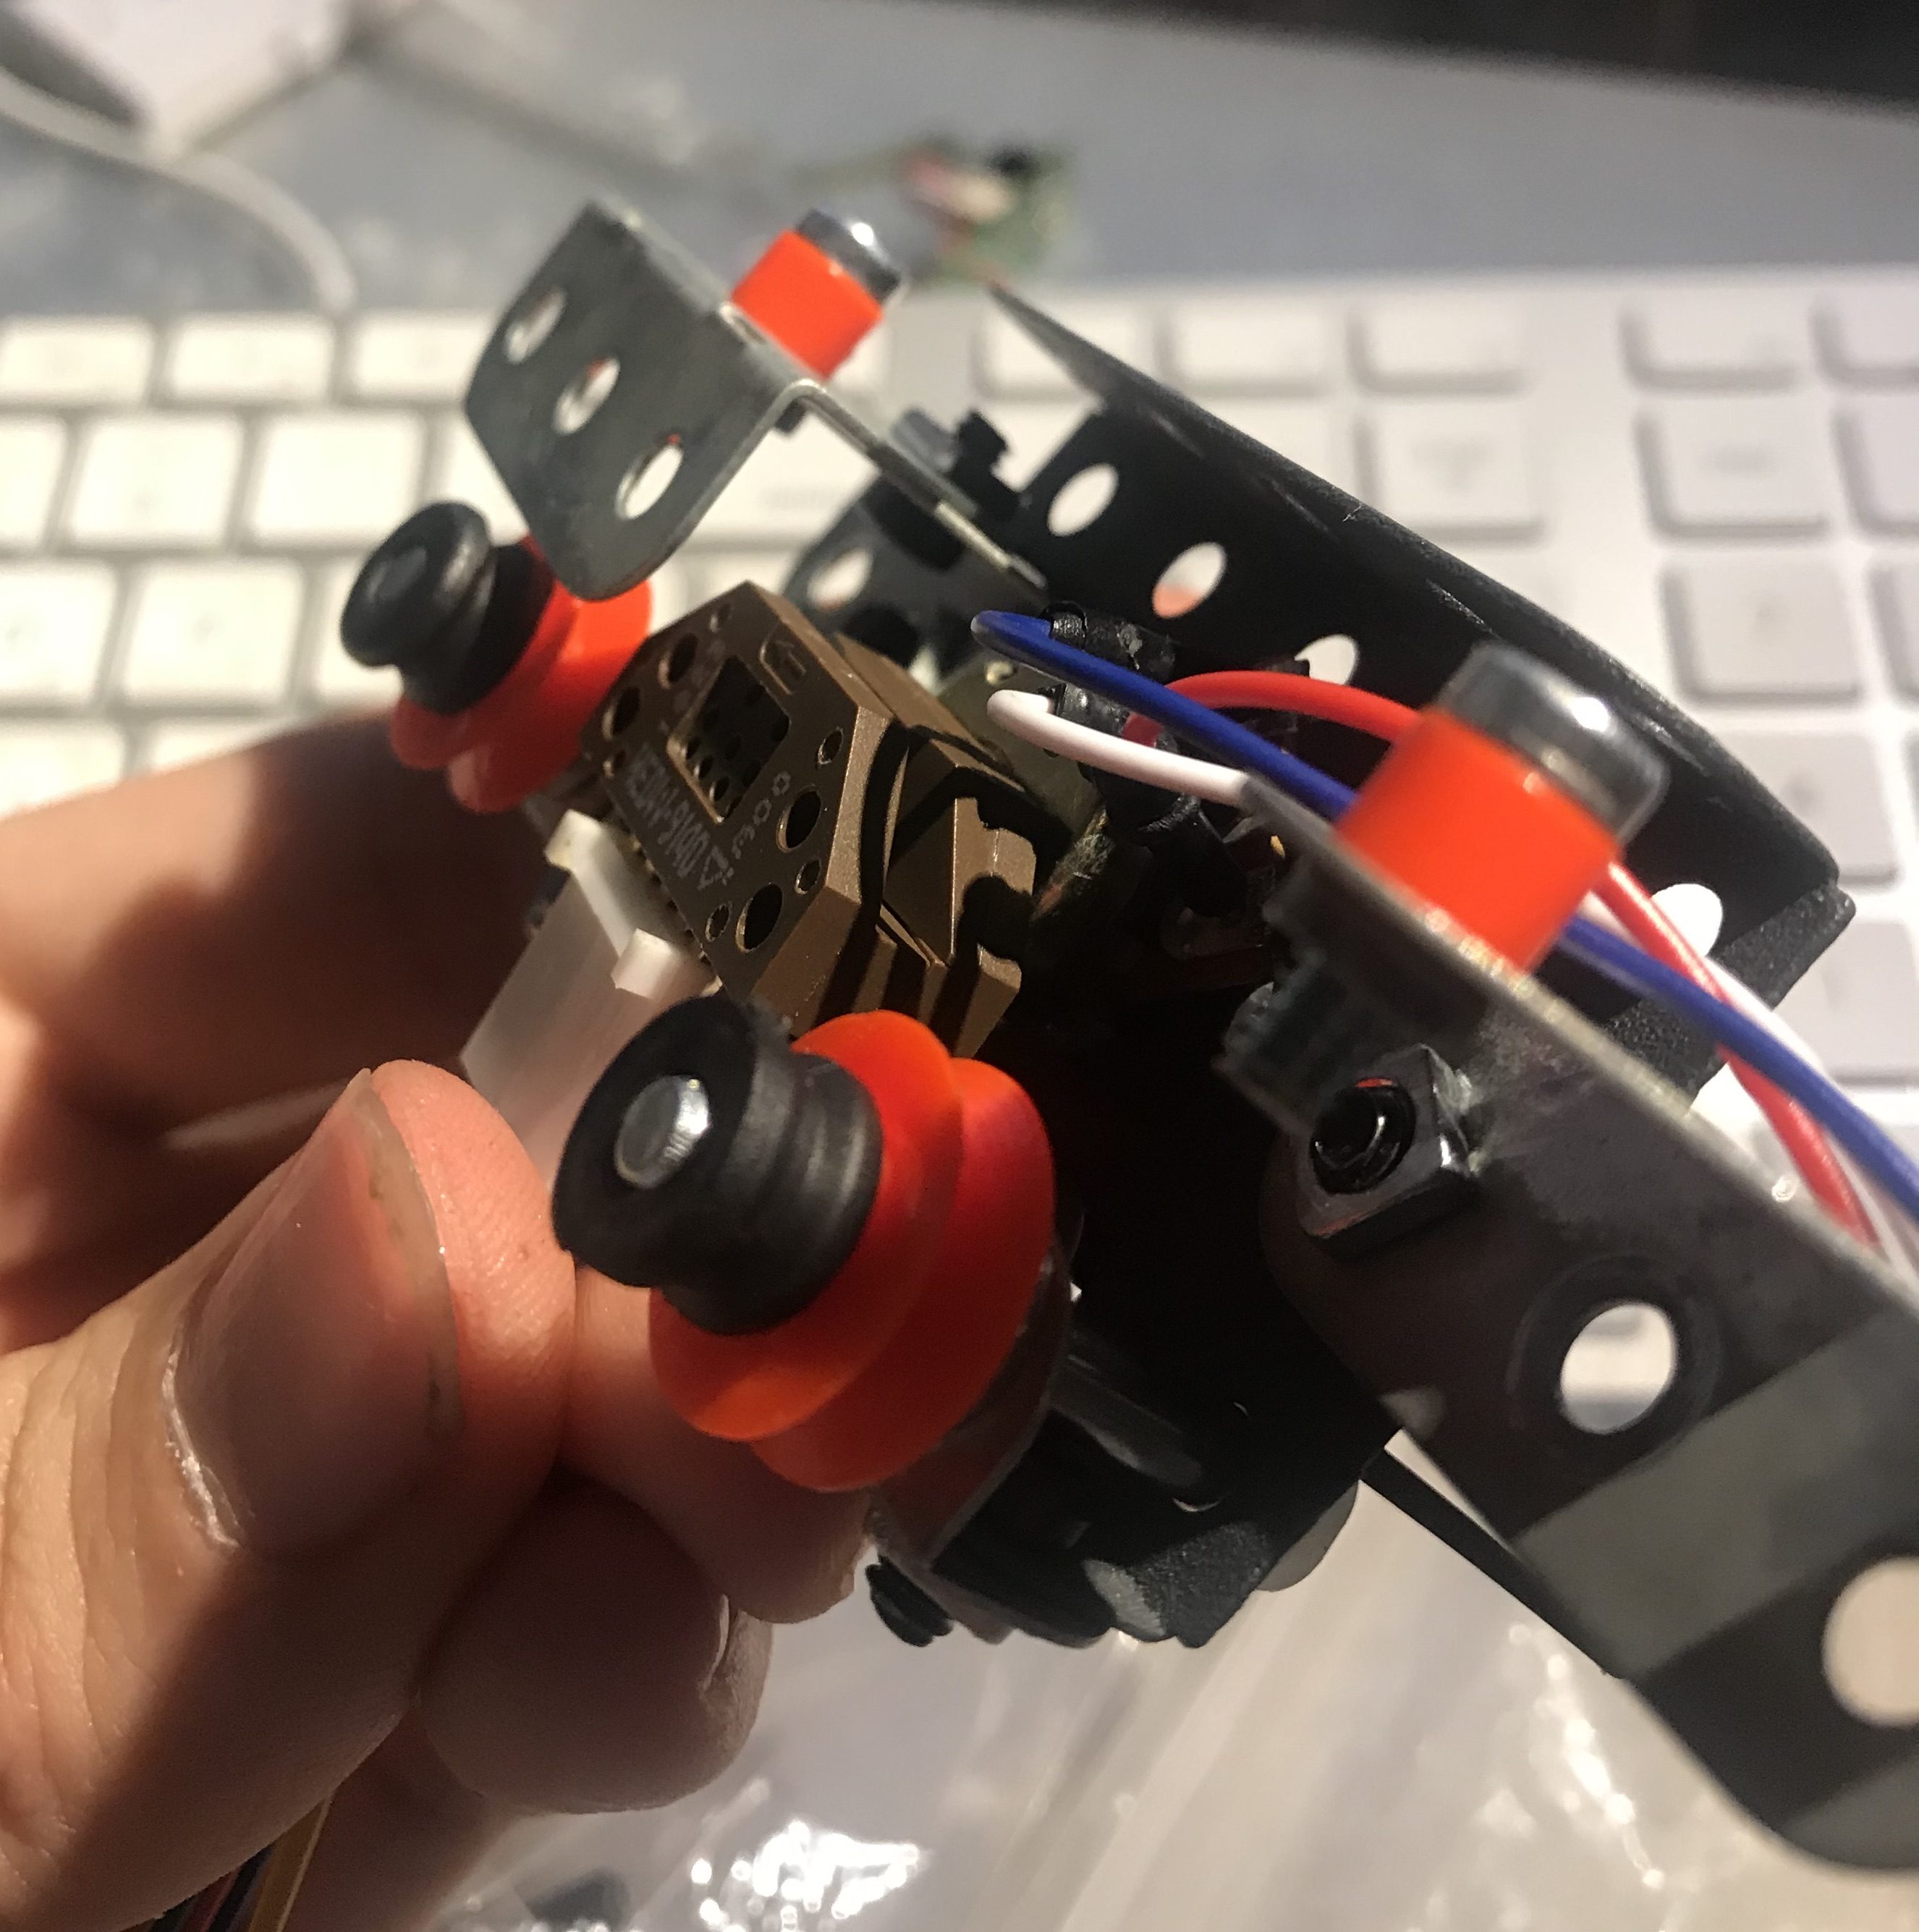
\includegraphics[width=1\linewidth]{figures/IMG_5871.jpg}
  \caption{Optical Encoder on Cart}
  \label{fig:cart2}
\end{subfigure}
\caption{Custom Built Low Friction Linear Guided Cart}
\end{figure}

\subsection{Software}
To develop the state space model analysis, software tools MATLAB and SIMULINK will be used. MATLAB to develop the system state model, test and implement observer based feedback control, and SIMULINK to simulate and test the system, as well as fine tune the control gains. Furthermore, the controllability and observability of the system can be assessed in MATLAB, and will be discussed in the final project report.

\section{Implementation Plan and Timeline}
\subsection{Timeline}
It has been decided upon that the project duration will last approximately 1 month, to ensure completion of the working control system before the due date. The following timeline shows the approximate estimated dates for each major phase of the project. It should be noted that some tasks will be completed in parallel rather than in series, when possible.\\

\begin{chronology}[5]{1}{30}{\textwidth}
\event{1}{Project Kick-off}
\event[1]{5}{Mechanical Setup}
\event[5]{8}{Wiring and Electronics}
\event[8]{11}{Integration Testing}
\event[11]{15}{Initialization (PWM, ADC, etc.)}
\event{15}{Individual Component Control Complete}
\event[15]{20}{BG Functions (Interrupts, ADC, etc.)}
\event{20}{System Implementation Complete}
\event[20]{25}{Control Model Development}
\event[25]{30}{Testing and Fine Tuning}
\event{30}{Project Deadline}
\end{chronology}
\textbf{Project Timeline for the Month of March, by Day}\\

\subsection{Software Implementation Approach}
An approximate approach to the functions that will run on the microcontroller have been discussed as follows:
\begin{itemize}
    \item Interrupt handler for optical encoder, triggered by channel A and B outputs. This ISR will increment or decrement the cart position according to the following figure values:
    \begin{figure}[H]
        \centering
        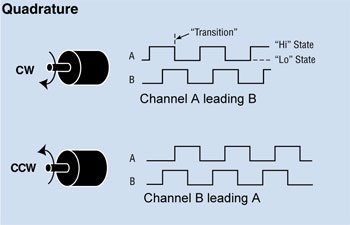
\includegraphics[width=.5\linewidth]{figures/quadrature.jpg}
        \caption{Quadrature Encoder Outputs \cite{quadref}}
        \label{fig:quad}
    \end{figure}
    \item Read ADC function for potentiometer input.
    \item Duty cycle set function to control the DC motor.
\end{itemize}
The aforementioned functions will be executed in the approximate following order, while the ISR is running in the background to vary the cart position:
\begin{enumerate}
    \item Check cart position.
    \item Read pendulum angle.
    \item Evaluate state feedback model control.
    \item Write PWM outputs for motor position.
    \item Repeat.
\end{enumerate}
\subsubsection{Concerns}
\label{conc}
There are a few potential roadblocks. Such issues may cause difficulty in programming the overall control system, especially due to the fact that our control model implies a substantial amount of pure theory, unlike a simple but effective PID controller. Said concerns are mentioned below:
\begin{itemize}
    \item Extremely fine optical encoder strip will result in rapid interrupts at high cart speeds. Could inhibit the control model from running in real time.
    \item Non-linearities such as friction will sufficiently impact the control model.
    \item Gain tuning takes time and testing, and producing a critically damped system will require accurate SIMULINK models and iterative physical testing.
\end{itemize}

\section{Conclusions}
Overall, this system is completely feasible, controllable and observable. Thorough testing has been completed with all proposed components to ensure satisfactory working requirements to implement the state controller. Furthermore, proposed GPIO for the microcontroller has been completed and checked in the course lab experiments, hence all the required knowledge is possessed. Moving forward, there are a few concerns that may cause potential problems in the execution of the project, as highlighted in section \ref{conc}. Such problems will be addressed as soon as possible once the integration of the functioning mechanical and electrical system before any controls development takes place.\newline

All to date development can be seen on Github \cite{github}, currently most development is on branch \textbf{init}. Folder \textbf{matlab/} discusses system analysis, controllability and observability. Folder \textbf{tiva/} contains all code for the microcontroller board and Code Composer Studio.

% ADD BIBLIOGRAPHY
\nocite{*}
\bibliographystyle{IEEE/IEEEtran}
\bibliography{IEEE/IEEEabrv,IEEE/biblio}

\end{document}
